% Beamer presentation
\documentclass[11pt,aspectratio=43,ignorenonframetext,t]{beamer}

% Presentation settings
\mode<presentation>{
  \usetheme[framenumber,titleframestart=1]{UoM_alex}
  \usefonttheme{professionalfonts} % using non standard fonts for beamer
  \usefonttheme{serif}
  \usepackage{fontspec}
  \setmainfont[Ligatures=TeX]{Arial}
}

% Handout settings
\mode<article>{
  \usepackage{fullpage}
  \usepackage{fontspec}
  \setmainfont[Ligatures=TeX]{Arial}
  \setlength{\parskip}{1.5\baselineskip} % correct beamer line spacings
  \setlength{\parindent}{0cm}
  \usepackage{enumitem}
  \setlist[itemize]{topsep=0pt}
}

 % Packages
\usepackage{graphicx}
\graphicspath{{./images/png}} % generic graphics path; overridden if necessary
\usepackage{amsmath}
\allowdisplaybreaks[1] % allow eqnarrays to break across pages
\usepackage{amssymb} 
\usepackage[HTML]{xcolor}
\definecolor{uomlinkblue}{HTML}{0071BC}
\usepackage{hyperref}
\hypersetup{
  colorlinks=true,
  linkcolor=uomlinkblue,
  filecolor=uomlinkblue,      
  urlcolor=uomlinkblue,
  pdflang={en-GB},
}
\usepackage[document]{ragged2e} % left aligned text for accessibility
\usepackage{tikz}
\usetikzlibrary{positioning, arrows, arrows.meta}
\usepackage{unicode-math} % unicode maths for accessibility
\usepackage{pdfcomment}   % for alt text for accessibility
\usepackage{rotating}     % allow portrait figures and tables
\usepackage{subfigure}    % allow matrices of figures
\usepackage{float}        % allows H option on floats to force here placement
\usepackage{multirow}     % allows merging of rows in tables
\usepackage{tabularx}     % allows fixed width tables
\usepackage{ctable}       % modifies \hline for use in table
\usepackage{bm}           % allow bold fonts in equations
\usepackage{pgf}          % allow graphics manipulation
\usepackage{etoolbox}
  
% Custom commands
\newcolumntype{Z}{>{\centering\arraybackslash}X}  % tabularx centered columns 

\makeatletter
  \DeclareRobustCommand{\em}
  {
    \@nomath\em
    \if b
      \expandafter\@car\f@series\@nil \normalfont
    \else
      \bfseries
    \fi
  }
\makeatother

\makeatletter
  \preto{\@verbatim}{\topsep=0pt \partopsep=0pt}
\makeatother

\def\checkmark{
  \tikz\fill[scale=0.4](0,.35) -- (.25,0) -- (1,.7) -- (.25,.15) -- cycle;
}

% Counters
\newcounter{example_number} % keep track of the example questions

% Frontmatter
\newcommand{\cmclecture}[1]{
  \title{Combinatorial Mesh Calculus (CMC): Lecture #1}
}
\author{
  Lectured by:
  \href{https://scholar.google.com/citations?user=x4R-snQAAAAJ&hl=en}
  {Dr. Kiprian Berbatov}$^1$\\
  \smallskip
  Lecture Notes Compiled by:
  \href{https://scholar.google.com/citations?user=CoIpITkAAAAJ&hl=en}
  {Muhammad Azeem}$^1$\\
  \smallskip
  Under the supervision of:
  \href{https://scholar.google.co.uk/citations?user=3nWJe5wAAAAJ&hl=en}
  {Prof. Andrey P. Jivkov}$^1$\\
  \smallskip
  {\tiny $^1$Department of Mechanical and Aerospace Engineering,
    The University of Manchester, Oxford Road, Manchester M13 9PL, UK}
}

% Special frames
\newcommand{\cmctitleframe}{
  \titlepage
  \begin{tikzpicture}[remember picture,overlay]
    \node[anchor=south east] at (current page.south east) {
      \href{https://youtube.com/@kipi.berbatov}{
        
\includegraphics[width=1.5cm]{youtube-icon.png}
      }
    };
  \end{tikzpicture}
}
\newcommand{\cmcendframe}{
  \begin{figure}
    \centering
    
\includegraphics[width=0.85\linewidth]{Thanks.png}
  \end{figure}
}

\cmclecture{8}
\date{24 October 2025}

\begin{document}

%========================= TITLE =========================
\begin{frame}
  \cmctitleframe
\end{frame}

\begin{frame}{Exterior Algebra}

\begin{block}{Graded-commutative rule.} If $A^\bullet=\bigoplus_{p\ge 0}A^p$ is a graded algebra and $v\in A^p$, $w\in A^q$, then

\begin{align*}
v\,w = (-1)^{pq}\,w\,v.
\end{align*}
\end{block}

\vspace{-0.3cm}
\begin{block}{Definition (Exterior algebra).}
Let $R$ be a CRWU and $V$ an $R$–module. The \emph{exterior algebra} $\Lambda^\bullet V$ is the smallest \emph{alternating} (associative, unital) $R$–algebra generated by $V$, i.e.\ the quotient of the tensor algebra $T(V)$ by the ideal generated by all $v\otimes v$ $(v\in V)$.
It is graded
\begin{align*}
\Lambda^\bullet V=\bigoplus_{p=0}^\infty \Lambda^p V,\qquad
\alpha\in\Lambda^p V,\ \beta\in\Lambda^q V \ \Rightarrow\ \alpha\wedge\beta\in\Lambda^{p+q}V,
\end{align*}

\end{block}
\end{frame}

\begin{frame}{Exterior Algebra}

\begin{block}{Definition (Exterior algebra).}
\vspace{-0.3cm}

\begin{align*}
\Lambda^\bullet V=\bigoplus_{p=0}^\infty \Lambda^p V,\qquad
\alpha\in\Lambda^p V,\ \beta\in\Lambda^q V \ \Rightarrow\ \alpha\wedge\beta\in\Lambda^{p+q}V,
\end{align*}
with $\Lambda^0V=R$, $\Lambda^1V=V$, and
\begin{align*}
\Lambda^2V=\left\{\sum_{k=1}^N \lambda_k\, v_k\wedge w_k \ \middle|\ N\in\mathbb{N},\ \lambda_k\in R,\ v_k,w_k\in V \right\}.
\end{align*}
The product is denoted by $\wedge$ and satisfies graded-commutativity: if $\alpha$ is homogeneous of degree $p$ and $\beta$ of degree $q$, then $\alpha\wedge\beta=(-1)^{pq}\beta\wedge\alpha$.
\end{block}
\end{frame}

\begin{frame}{Basic anti-commutation with a vector}
\begin{block}{Proposition.}
Let $R$ be a CRWU, $V$ an $R$–module, $v\in V=\Lambda^1V$ and $\alpha\in\Lambda^\bullet V$ homogeneous of degree $p$. Then
\begin{align*}
v\wedge\alpha = (-1)^p\,\alpha\wedge v.
\end{align*}
In particular $v\wedge v=0$ and, if $p$ is odd, $v\wedge\alpha+\alpha\wedge v=0$.
\end{block}
\vspace{-0.2cm}
\begin{proof}
In $\Lambda^\bullet V$ we have the graded-commutative law with degrees $\deg v=1$ and $\deg\alpha=p$, hence $v\wedge\alpha=(-1)^{1\cdot p}\alpha\wedge v$. Taking $p=1$ yields $v\wedge v=-\,v\wedge v$, so $2(v\wedge v)=0$. Since $v\wedge v$ is the image of $v\otimes v$ in the quotient $T(V)/\langle v\otimes v\rangle$, we have $v\wedge v=0$ by construction (no characteristic assumption needed). If $p$ is odd, $(-1)^p=-1$ and $v\wedge\alpha+\alpha\wedge v=0$.
\end{proof}
\end{frame}

\begin{frame}{Dimension bounds and spanning sets}
\begin{block}{Corollary (Finite rank $n$).}
Let $R$ be a CRWU and $V$ a free $R$–module of rank $n$ with basis $e_1,\dots,e_n$. Then:
\begin{enumerate}
\item If $p>n$, then $\Lambda^p V=0$.
\item If $1\le p\le n$, then the $p$–vectors
\begin{align*}
\{\, e_{i_1}\wedge e_{i_2}\wedge\cdots\wedge e_{i_p}\mid 1\le i_1<\cdots<i_p\le n \,\}
\end{align*}
span $\Lambda^p V$.
\end{enumerate}
\end{block}
\end{frame}

\begin{frame}{Proof}
\begin{proof}
(1) Any pure $p$–tensor $v_1\wedge\cdots\wedge v_p$ is alternating and multilinear in the $v_k$. Express $$v_k=\sum_{j=1}^n \lambda_{kj}e_j$$ and expand. Every term containing a repeated basis vector $e_j$ vanishes because $e_j\wedge e_j=0$. With only $n$ distinct basis vectors available, no nonzero terms remain when $p>n$.\\

(2) By multilinearity, each $v_1\wedge\cdots\wedge v_p$ is an $R$–linear combination of wedges of the basis vectors. Using $e_i\wedge e_j=-\,e_j\wedge e_i$ we can sort factors to increasing indices; terms with repeats vanish. Hence the displayed set spans $\Lambda^pV$.
\end{proof}
\end{frame}


\begin{frame}{Example in $\mathbb{R}^2$: wedge and determinants}
\vspace{-0.3cm}
Let $V=\mathbb{R}^2$ with basis $e_1=(1,0)$, $e_2=(0,1)$. Take
\begin{align*}
u&=\lambda_1 e_1+\lambda_2 e_2,\qquad
v=\mu_1 e_1+\mu_2 e_2,\qquad
w=\kappa_1 e_1+\kappa_2 e_2.
\end{align*}
\textbf{Compute $u\wedge v$.} Using bilinearity and $e_1\wedge e_1=e_2\wedge e_2=0$, $e_2\wedge e_1=-\,e_1\wedge e_2$,
\begin{align*}
u\wedge v
&=(\lambda_1 e_1+\lambda_2 e_2)\wedge(\mu_1 e_1+\mu_2 e_2)\\
&=\lambda_1\mu_2\, (e_1\wedge e_2)+\lambda_2\mu_1\, (e_2\wedge e_1)\\
&=(\lambda_1\mu_2-\lambda_2\mu_1)\, e_1\wedge e_2
= \det\!\begin{pmatrix}\lambda_1&\lambda_2\\ \mu_1&\mu_2\end{pmatrix}\, e_1\wedge e_2.
\end{align*}
\textbf{Compute $u\wedge v\wedge w$.} Since $\Lambda^3\mathbb{R}^2=0$ (corollary with $p=3>2$),
\begin{align*}
u\wedge v\wedge w = 0.
\end{align*}
The scalar coefficient of $e_1\wedge e_2$ is the signed area (determinant) of the $2\times 2$ matrix with rows (or columns) $u,v$; the third wedge vanishes because at most two independent directions live in $\mathbb{R}^2$.
\end{frame}

\begin{frame}{Example in $\mathbb{R}^3$: cross and triple products}
\vspace{-0.2cm}
Let $V=\mathbb{R}^3$ with basis $e_1,e_2,e_3$. Write
\begin{align*}
u&=\lambda_1 e_1+\lambda_2 e_2+\lambda_3 e_3,\\
v&=\mu_1 e_1+\mu_2 e_2+\mu_3 e_3,\\
w&=\kappa_1 e_1+\kappa_2 e_2+\kappa_3 e_3.
\end{align*}
\textbf{$u\wedge v$.} Expand and collect on the basis $\{e_1\wedge e_2,\ e_2\wedge e_3,\ e_3\wedge e_1\}$:
\begin{align*}
u\wedge v
=&(\lambda_1\mu_2-\lambda_2\mu_1)\, e_1\wedge e_2
+(\lambda_2\mu_3-\lambda_3\mu_2)\, e_2\wedge e_3\\
&
+(\lambda_3\mu_1-\lambda_1\mu_3)\, e_3\wedge e_1.
\end{align*}
\textbf{Identification with the cross product.} Using the canonical isomorphism $\ast:\Lambda^2\mathbb{R}^3\to\mathbb{R}^3$ defined by
\begin{align*}
\ast(e_2\wedge e_3)=e_1,\quad \ast(e_3\wedge e_1)=e_2,\quad \ast(e_1\wedge e_2)=e_3,
\end{align*}
\textbf{Note:} We will discuss this \textit{canonical isomorphism ($\ast$)} in coming lectures.
\end{frame}


\begin{frame}{Example in $\mathbb{R}^3$: cross and triple products}
\begin{block}{}
We get
\begin{align*}
\ast(u\wedge v)=
\begin{pmatrix}
\lambda_2\mu_3-\lambda_3\mu_2\\
\lambda_3\mu_1-\lambda_1\mu_3\\
\lambda_1\mu_2-\lambda_2\mu_1
\end{pmatrix}
= u\times v.
\end{align*}

\textbf{$u\wedge v\wedge w$.} Expanding on the basis $e_1\wedge e_2\wedge e_3$ yields
\begin{align*}
u\wedge v\wedge w
= \det\!\begin{pmatrix}
\lambda_1 & \lambda_2 & \lambda_3\\
\mu_1     & \mu_2     & \mu_3\\
\kappa_1  & \kappa_2  & \kappa_3
\end{pmatrix}\, e_1\wedge e_2\wedge e_3.
\end{align*}
The scalar is the scalar triple product $(u\times v)\cdot w$; it gives the oriented volume of the parallelepiped spanned by $(u,v,w)$.
\end{block}

\end{frame}

\begin{frame}{Bases of $\Lambda^\bullet \mathbb{R}^2$ and $\Lambda^\bullet \mathbb{R}^3$}
\begin{block}{}
    \textbf{For $V=\mathbb{R}^2$ with basis $e_1,e_2$:}
\begin{align*}
\Lambda^\bullet V
=& \Lambda^0 V \ \oplus\ \Lambda^1 V \ \oplus\ \Lambda^2 V\\
=& \operatorname{Span}\{1\}\ \oplus\ \operatorname{Span}\{e_1,e_2\}\ \oplus\ \operatorname{Span}\{e_1\wedge e_2\}.
\end{align*}

\textbf{For $V=\mathbb{R}^3$ with basis $e_1,e_2,e_3$:}
\begin{align*}
\Lambda^\bullet V
=& \Lambda^0 V \oplus \Lambda^1 V \oplus \Lambda^2 V \oplus \Lambda^3 V\\
&= \operatorname{Span}\{1\}
\ \oplus\ \operatorname{Span}\{e_1,e_2,e_3\}
\\& \oplus\ \operatorname{Span}\{e_1\wedge e_2,\ e_2\wedge e_3,\ e_1\wedge e_3\}\\
&\quad\oplus\ \operatorname{Span}\{e_1\wedge e_2\wedge e_3\}.
\end{align*}
\end{block}

\end{frame}


%==============================%
% Exterior Algebra: Bases, Exterior Powers, Determinant, Interior Product
%==============================%

\begin{frame}{Basis of $\Lambda^{p}V$ and Binomial Count}
\begin{block}{Theorem.}
Let $R$ be a CRWU and $V$ an $n$–dimensional free $R$–module with basis $e_1,\dots,e_n$. For $p\in\{0,1,\dots,n\}$ the set
\begin{align*}
\mathcal{B}_{p}\;=\;\{\, e_{i_1}\wedge e_{i_2}\wedge\cdots\wedge e_{i_p}\mid 1\le i_1<\cdots<i_p\le n \,\}
\end{align*}
is a basis of $\Lambda^{p}V$. In particular,
\begin{align*}
\dim\Lambda^{p}V=\binom{n}{p}.
\end{align*}
\end{block}

\end{frame}

\begin{frame}{Basis of $\Lambda^{p}V$ and Binomial Count}
\begin{proof}
\emph{Spanning:} Any $v_1\wedge\cdots\wedge v_p$ expands $R$–linearly in the basis $\{e_j\}$; terms with repeated indices vanish ($e_i\wedge e_i=0$), and the graded–commutativity lets us sort indices increasingly, giving a combination of elements of $\mathcal{B}_p$.
\emph{Linear independence:} Consider the coordinate map $\phi:\Lambda^pV\!\to\! R^{\binom{n}{p}}$ that records coefficients w.r.t.\ $\mathcal{B}_p$; by construction its kernel is $0$, so the family is independent.
\end{proof}

\textbf{Binomial theorem and dimensions.}
For $t$ an indeterminate,
\begin{align*}
\sum_{p=0}^{n}\dim\Lambda^{p}V\; t^{p}
=\sum_{p=0}^{n}\binom{n}{p}t^{p}=(1+t)^{n}.
\end{align*}
At $t=1$ this gives $\sum_{p=0}^n\binom{n}{p}=2^n=\dim\Lambda^{\bullet}V$.
\end{frame}

%------------------------------%
\begin{frame}{Exterior Power of a Linear Map}
\begin{block}{Definition.}
Let $R$ be a CRWU, $V,W$ $R$–modules, $p\in\mathbb{N}$, and $f\in \operatorname{Hom}_R(V,W)$. The \emph{$p$–th exterior power}
\begin{align*}
\Lambda^{p}f:\operatorname{Hom}_{R}\left(\Lambda^{p}V, \Lambda^{p}W\right)
\end{align*}
is the unique $R$–linear map determined on decomposables by
\begin{align*}
(\Lambda^{p}f)(v_1\wedge\cdots\wedge v_p)=f(v_1)\wedge\cdots\wedge f(v_p).
\end{align*}
Uniqueness follows from multi\-linearity and alternation.
\end{block}
\end{frame}

\begin{frame}{Exterior Power of a Linear Map}

\begin{block}{Example ($V=W=\mathbb{R}^2$).}
Let $e_1=(1,0)$, $e_2=(0,1)$ and write
\begin{align*}
f(e_1)=a_{11}e_1+a_{21}e_2,\qquad f(e_2)=a_{12}e_1+a_{22}e_2.
\end{align*}
Then
\begin{align*}
(\Lambda^2 f)(e_1\wedge e_2)
&= f(e_1)\wedge f(e_2)\\
&=(a_{11}e_1+a_{21}e_2)\wedge (a_{12}e_1+a_{22}e_2)\\
&=(a_{11}a_{22}-a_{21}a_{12})\, e_1\wedge e_2
=\det\!\begin{pmatrix}a_{11}&a_{12}\\ a_{21}&a_{22}\end{pmatrix}\, e_1\wedge e_2.
\end{align*}
\end{block}
\end{frame}

%------------------------------%
\begin{frame}{Determinant via Top Exterior Power}
\vspace{-0.3cm}
\begin{block}{Definition (Endomorphism).}
$\operatorname{End}_R(V)=\operatorname{Hom}_R(V,V)$ is the $R$–algebra of $R$–linear maps $V\to V$.
\end{block}

\vspace{-0.3cm}
\begin{block}{Top exterior power and determinant.}
If $\dim V=n$, then $\dim\Lambda^{n}V=\binom{n}{n}=1$, so $\Lambda^{n}f:\Lambda^{n}V\to\Lambda^{n}V$ is multiplication by a unique scalar $\lambda\in R$:
\begin{align*}
(\Lambda^{n}f)(\alpha)=\lambda\,\alpha,\qquad \alpha\in\Lambda^{n}V.
\end{align*}
We define $\det(f):=\lambda$.

\textbf{Compatibility with matrices.}
Let $e=(e_1,\dots,e_n)$ be a basis and $A=(f)^e_e\in M_{n\times n}(R)$ the matrix of $f$. Then
\begin{align*}
\det(f)=\det(A).
\end{align*}
\end{block}
\end{frame}

\begin{frame}{Determinant via Top Exterior Power}
\begin{proof}[Proof sketch with details on $e_1\wedge\!\cdots\!\wedge e_n$]
Write $f(e_j)=\sum_{i}a_{ij}e_i$. Then
\begin{align*}
(\Lambda^n f)(e_1\wedge\cdots\wedge e_n)
&=\bigwedge_{j=1}^n\left(\sum_{i=1}^n a_{ij}e_i\right)\\
&
= \sum_{\sigma\in S_n}\!\left(\operatorname{sgn}\sigma\right)\, a_{1\sigma(1)}\cdots a_{n\sigma(n)} \, e_1\wedge\cdots\wedge e_n\\
&=(\det A)\, e_1\wedge\cdots\wedge e_n,
\end{align*}
so $\Lambda^n f$ is multiplication by $\det A$.
\end{proof}
\end{frame}

%------------------------------%
\begin{frame}{Multiplicativity of Determinant}
\textbf{Theorem.}
Let $R$ be a CRWU, $\dim V=n$, and $f,g\in\operatorname{End}_R(V)$. Then
\begin{align*}
\det(g\circ f)=\det(g)\cdot \det(f).
\end{align*}
\vspace{-0.6cm}
\begin{proof}
Functoriality of exterior powers gives $\Lambda^{n}(g\circ f)=\Lambda^{n}g\circ \Lambda^{n}f$. Since $\Lambda^{n}V$ is $1$–dimensional, there exist unique $\lambda,\mu\in R$ with
\begin{align*}
\Lambda^{n}f=\lambda\,\mathrm{id},\qquad \Lambda^{n}g=\mu\,\mathrm{id}.
\end{align*}
Hence
\begin{align*}
\Lambda^{n}(g\circ f)=(\Lambda^{n}g)\circ(\Lambda^{n}f)=(\mu\,\mathrm{id})\circ(\lambda\,\mathrm{id})=(\mu\lambda)\,\mathrm{id},
\end{align*}
so $\det(g\circ f)=\mu\lambda=\det(g)\det(f)$.
\end{proof}
\end{frame}

\begin{frame}{Visualization}
    \begin{center}
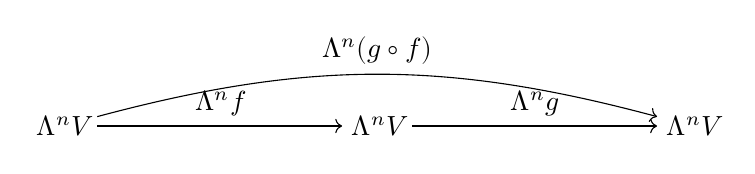
\begin{tikzpicture}
    % Define nodes
    \node (L1) at (0,0) {$\Lambda^n V$};
    \node (L2) at (4,0) {$\Lambda^n V$};
    \node (L3) at (8,0) {$\Lambda^n V$};

    % Draw arrows
    \draw[->] (L1) -- node[above] {$\Lambda^n f$} (L2);
    \draw[->] (L2) -- node[above] {$\Lambda^n g$} (L3);
    \draw[->, bend left=15] (L1) to node[above] {$\Lambda^n(g\circ f)$} (L3);
\end{tikzpicture}
\end{center}
\end{frame}

%------------------------------%
\begin{frame}{Interior Product (Contraction)}
\begin{block}{Definition.}
Let $R$ be a CRWU, $V$ an $R$–module. For $p\ge 1$, the \emph{interior product} (contraction)
\begin{align*}
i:\; V\times \Lambda^{p}V^{*}\longrightarrow \Lambda^{p-1}V^{*},\qquad (v,\omega)\mapsto i_v\omega
\end{align*}
is the unique $R$–bilinear map such that:
\begin{align*}
\text{(1) } &p=1:\quad i_v w = w(v)\in R,\qquad (v\in V,\ w\in V^*);\\
\text{(2) } &\text{Leibniz rule (degree $-1$ derivation): }\\
& i_v(\omega\wedge\eta)=i_v\omega\wedge \eta+(-1)^{p}\,\omega\wedge i_v\eta,\\
&\text{for }\omega\in\Lambda^{p}V^*,\ \eta\in\Lambda^{q}V^*.
\end{align*}
By $R$–bilinearity, extend to all $p$ and sums.
\end{block}

\end{frame}

%------------------------------%
\begin{frame}{Interior Product: Computations in $\mathbb{R}^2$}
Let $V=\mathbb{R}^2$ with basis $e_1,e_2$ and dual basis $e^1,e^2$.

\textbf{On $1$–forms:}
\begin{align*}
i_{e_1}(e^1)=1,\quad i_{e_1}(e^2)=0,\qquad
i_{e_2}(e^1)=0,\quad i_{e_2}(e^2)=1.
\end{align*}

\textbf{On $2$–forms:} using $i_v(\omega\wedge\eta)=i_v\omega\wedge\eta- \omega\wedge i_v\eta$ for $\omega\in\Lambda^1$,
\begin{align*}
i_{e_1}(e^1\wedge e^2)&=i_{e_1}(e^1)\wedge e^2 - e^1\wedge i_{e_1}(e^2)= 1\cdot e^2 - e^1\wedge 0 = e^2,\\
i_{e_2}(e^1\wedge e^2)&=i_{e_2}(e^1)\wedge e^2 - e^1\wedge i_{e_2}(e^2)= 0\cdot e^2 - e^1\cdot 1 = -\,e^1.
\end{align*}
For $v=a e_1+b e_2$,
\begin{align*}
i_{v}(e^1\wedge e^2)= a\,e^2 - b\,e^1.
\end{align*}
This is the Hodge–dual of $v$ in dimension $2$.

\textbf{On functions ($0$–forms):} $i_v\colon \Lambda^0 V^*=R\to 0$ is the zero map.
\end{frame}



%------------------------------%


\begin{frame}{Algebraic Identities for the Interior Prod.}
\vspace{-0.3cm}
\begin{block}{Proposition.}
Let $R$ be a CRWU and $V$ an $R$–module.
\begin{enumerate}
\item For any $v\in V$, $i_v\circ i_v=0$ on $\Lambda^{\bullet}V^*$.
\item The canonical map
\begin{align*}
\phi:\Lambda^{p}(V^{*})\longrightarrow (\Lambda^{p}V)^{*}
\end{align*}
defined on decomposables by
\begin{align*}
\phi(w_1\wedge\cdots\wedge w_p)(v_1\wedge\cdots\wedge v_p)
= i_{v_p}\circ\cdots\circ i_{v_1}(w_1\wedge\cdots\wedge w_p)
\end{align*}
is an isomorphism when $V$ is finite free. Equivalently,
\begin{align*}
\phi(w_1\wedge\cdots\wedge w_p)(v_1\wedge\cdots\wedge v_p)
=\det\!\left(w_i(v_j)\right)_{1\le i,j\le p}.
\end{align*}
\end{enumerate}
\end{block}
\end{frame}

\begin{frame}{Proof}
    \begin{proof}
(1) It suffices to check on $\omega=w_1\wedge\cdots\wedge w_p$ with $w_i\in V^*$. The operator $i_v$ inserts $v$ into the first slot of the alternating $p$–form (up to signs).\\
Inserting the same vector twice yields $0$ by alternation, hence $i_v^2\omega=0$; linearity gives the claim.\\

(2) For decomposables the two displayed formulas agree (straight computation using the Leibniz rule shows the cofactor expansion).\\
In a basis $\{e_i\}$ with dual $\{e^i\}$, both $\Lambda^{p}(V^*)$ and $(\Lambda^{p}V)^*$ have the same rank $\binom{n}{p}$, and $\phi$ sends the basis element $e^{i_1}\wedge\cdots\wedge e^{i_p}$ to the functional that picks the coefficient of $e_{i_1}\wedge\cdots\wedge e_{i_p}$; hence $\phi$ is bijective.
\end{proof}
\end{frame}

%------------------------------%
\begin{frame}{Worked Contraction Example}
For $w_1,w_2\in V^*$ and $v_1,v_2\in V$,
\begin{align*}
i_{v_2}\circ i_{v_1}(w_1\wedge w_2)
&= i_{v_2}\left( i_{v_1}(w_1)\wedge w_2 - w_1\wedge i_{v_1}(w_2)\right)\\
&= i_{v_2}(w_1(v_1))\, w_2 \;-\; i_{v_2}(w_1)\, w_2(v_1) \;-\; i_{v_2}(w_2(v_1))\, w_1 \;+\; i_{v_2}(w_2)\, w_1(v_1)\\
&= 0 \cdot w_2 \;-\; w_1(v_2)\, w_2(v_1) \;-\; 0 \cdot w_1 \;+\; w_2(v_2)\, w_1(v_1)\\
&= \begin{vmatrix}
w_1(v_1) & w_1(v_2)\\
w_2(v_1) & w_2(v_2)
\end{vmatrix}.
\end{align*}
Thus, for $p=2$,
\begin{align*}
\phi(w_1\wedge w_2)(v_1\wedge v_2)=\det\!\begin{pmatrix}
w_1(v_1) & w_1(v_2)\\
w_2(v_1) & w_2(v_2)
\end{pmatrix},
\end{align*}
which matches the determinant–via–top–exterior–power paradigm.
\end{frame}

\begin{frame}{Summary of Lecture 07}
\vspace{-0.3cm}
\begin{block}{Main Ideas: Exterior Algebra and Determinant Structures}
\begin{itemize}
  \item \textbf{Exterior algebra $\Lambda^{\bullet}V$}: smallest alternating, associative, unital algebra generated by a module $V$ over a CRWU.
  \item It is a \textbf{graded algebra}:
  \vspace{-0.4cm}
  \begin{align*}
  \Lambda^{\bullet}V = \bigoplus_{p=0}^{n} \Lambda^{p}V, \quad
  \alpha\in\Lambda^{p}V, \ \beta\in\Lambda^{q}V \Rightarrow
  \alpha\wedge\beta=(-1)^{pq}\beta\wedge\alpha.
  \end{align*}
  \item \textbf{Basis:} For $\dim V=n$, $\{e_{i_1}\wedge\cdots\wedge e_{i_p}\mid 1\le i_1<\cdots<i_p\le n\}$ is a basis of $\Lambda^{p}V$.
  \item \textbf{Dimension:} $\dim\Lambda^{p}V=\binom{n}{p}$, and
  \vspace{-0.4cm}
  \begin{align*}
  \sum_{p=0}^{n}\dim\Lambda^{p}V\;t^p = (1+t)^{n}.
  \end{align*}
\end{itemize}
\end{block}
\end{frame}

\begin{frame}{Summary of Lecture 07}
\begin{block}{Main Ideas: Exterior Algebra and Determinant Structures}
\begin{itemize}
  \item \textbf{Exterior power of maps:} $\Lambda^{p}f(v_1\wedge\cdots\wedge v_p)=f(v_1)\wedge\cdots\wedge f(v_p)$.
  \item \textbf{Determinant:} For $f\in\mathrm{End}(V)$, $\Lambda^{n}f$ acts on the one-dimensional $\Lambda^{n}V$ by multiplication with $\det(f)$, and $\det(g\circ f)=\det(g)\det(f)$.
  \item \textbf{Interior product:} $i_v:\Lambda^{p}V^*\to\Lambda^{p-1}V^*$ defined by
  \begin{align*}
  i_v(\omega\wedge\eta)=i_v\omega\wedge\eta+(-1)^{p}\omega\wedge i_v\eta,\quad i_vw=w(v).
  \end{align*}
  \item \textbf{Canonical isomorphism:} $\Lambda^{p}(V^*)\cong(\Lambda^{p}V)^*$, with
  \begin{align*}
  \phi(w_1\wedge\cdots\wedge w_p)(v_1\wedge\cdots\wedge v_p)=
  \det\!\big(w_i(v_j)\big)_{1\le i,j\le p}.
  \end{align*}
\end{itemize}
\end{block}
\end{frame}

\begin{frame}{Roadmap}
\begin{center}
\vspace{-1.5cm}
\hspace{-1.0cm}
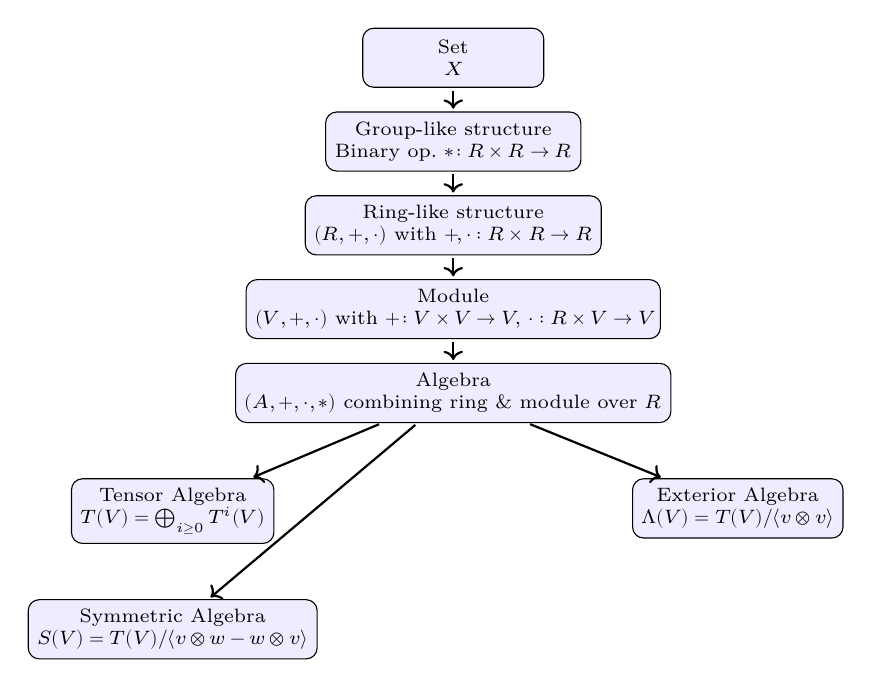
\begin{tikzpicture}[
  node distance=0.3cm and 1.1cm,
  every node/.style={align=center, font=\scriptsize},
  box/.style={draw, rounded corners, fill=blue!7, minimum width=2.3cm, minimum height=0.75cm},
  arrow/.style={->, thick, shorten >=1pt, shorten <=1pt}
  ]

\node[box] (set) {Set \\ $X$};
\node[box, below=of set] (group) {Group-like structure \\ Binary op.\ $*\!:R\times R\to R$};
\node[box, below=of group] (ring) {Ring-like structure \\ $(R,+,\cdot)$ with $+\!,\cdot:R\times R\to R$};
\node[box, below=of ring] (module) {Module \\ $(V,+,\cdot)$ with $+\!:V\times V\to V$, $\cdot:R\times V\to V$};
\node[box, below=of module] (algebra) {Algebra \\ $(A,+,\cdot,\ast)$ combining ring \& module over $R$};
\node[box, below left=0.7cm and -0.5cm of algebra] (tensor) {Tensor Algebra \\ $T(V)=\bigoplus_{i\ge0}T^i(V)$};
\node[box, below=0.7cm of tensor] (symmetric) {Symmetric Algebra \\ $S(V)=T(V)/\langle v\otimes w-w\otimes v\rangle$};
\node[box, below right=0.7cm and -0.5cm of algebra] (exterior) {Exterior Algebra \\ $\Lambda(V)=T(V)/\langle v\otimes v\rangle$};

\draw[arrow] (set) -- (group);
\draw[arrow] (group) -- (ring);
\draw[arrow] (ring) -- (module);
\draw[arrow] (module) -- (algebra);
\draw[arrow] (algebra) -- (tensor);
\draw[arrow] (algebra) -- (symmetric);
\draw[arrow] (algebra) -- (exterior);
%\node[below=0.2cm of symmetric] (caption);
\end{tikzpicture}
\end{center}
\end{frame}


\begin{frame}{Thanks}
  \cmcendframe
\end{frame}

\end{document}
